
\documentclass[sigchi]{acmart}

\settopmatter{printacmref=false, printccs=true, printfolios=true}
%%
%% \BibTeX command to typeset BibTeX logo in the docs
\AtBeginDocument{%
  \providecommand\BibTeX{{%
    \normalfont B\kern-0.5em{\scshape i\kern-0.25em b}\kern-0.8em\TeX}}}

%% Rights management information.  This information is sent to you
%% when you complete the rights form.  These commands have SAMPLE
%% values in them; it is your responsibility as an author to replace
%% the commands and values with those provided to you when you
%% complete the rights form.
\setcopyright{none}
%\copyrightyear{none}
\acmYear{2021}
\acmDOI{}

%% These commands are for a PROCEEDINGS abstract or paper.
\acmConference[Technical Report]{May}{{\today}}{Cologne, Germany}
\acmBooktitle{}
\acmPrice{}
\acmISBN{}

\usepackage{subfig}
\usepackage[english, german]{babel}
\begin{document}

\title{The impact of the avatar representation on team trust and effectiveness in a shared virtual environment.}

\author{Hannes Hinrichs}
\email{hhinrich@smail.th-koeln.de}
\affiliation{%
  \institution{TH-Köln}
  \city{Cologne}
  \country{Germany}
}

\begin{abstract}
The goal of this work is to find out if different avatar representations have an impact on the formed trust and effectiveness of a team. The first question here is whether an inverse-kinematic human-like representation or an abstract non-human-like representation is more effective in generating trust in a newly formed virtual team. The second question addresses whether the trust formed by the different representations influences the effectiveness of the virtual team. To answer these questions, a quantitative study was conducted in which different participants in a three-person team performed a collaborative task in a shared virtual environment. No significant differences in effectiveness were found between the teams. The results of the study also show that in the threeperson team significantly more trust was built with non humanlike avatars. Furthermore, with non-human-like avatars there was a significant relationship between the cognitive trust formed and teameffectiveness. This means that the simplicity of a non-human-like avatar in a newly formed team in a shared virtual environment can be effective in creating a trusting work atmosphere.
\end{abstract}

\keywords{Virtual-Reality, Trust, Team formation, virtual Team, Avatar}

%% A "teaser" image appears between the author and affiliation
%% information and the body of the document, and typically spans the
%% page.
\begin{teaserfigure}
  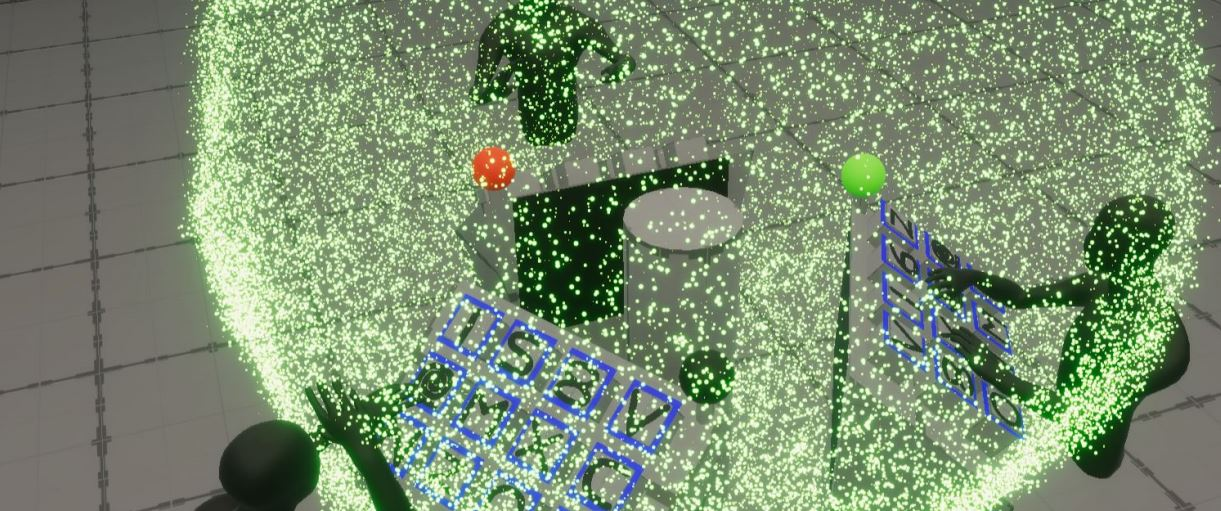
\includegraphics[width=\textwidth]{Abbildungen/RoundSuccsessful2}
  \caption{This figure represents the developed Shared-Virual-Environment with the participants infront of there Podests. A green sphere appears clearly visible when a round is successfully completed.}
  \Description{This figure represents the developed Shared-Virual-Environment. The green sphere appears clearly visible for all participants when a round is successfully completed.}
  \label{fig:teaser}
\end{teaserfigure}

%%
%% This command processes the author and affiliation and title
%% information and builds the first part of the formatted document.
\maketitle

\section{INTRODUCTION}
With advancing technological development, digital communication is becoming more and more central. Companies around the world have long relied on overcoming spatial and temporal boundaries.
New generations of social networking systems are being created on the premise of improving communication to remote individuals.
Einsatzfelder sind beispielsweise die Mobil- und Internettelefonie, die FOIP/VOIP- Telefonkonferenzen oder die sozialen virtuellen 3D- Umgebungen.
All these technologies share the goal of enhancing social presence, allowing users to gain some degree of insight and the cognitive and affective states of the interaction partner \citep[S. 407–447]{biocca2001plugging}.
Employees in an organization are very often not in the same place, yet many companies still want their teams to be effective \citep[S. 791-792]{jarvenpaa1999communication}. \textit{Virtual teams} can provide a remedy here. 
Before the Corona pandemic, in Q2 2020, 4\% of all employees in Germany worked from home. This share has risen to 24\% over the course of the year - as of 01.01.2021 - and theoretically 80\% of employees could work from home. \citep{statistaCorona2020}. As a result of this development, companies have inevitably had to look at how virtual teams work.
When a virtual team meets in a virtual reality environment, avatars can be used to represent the individual. These are used to interact and communicate with other participants in the shared virtual environment.
\textit{Virtual teams} are often short-lived, which creates a deficit in the trust formed with team members.
Working in a geographically separated team that does not trust each other or does not work together properly inhibits its performance. \citep[S. 98-107]{huang1998supporting} \citep[S. 399-417]{turoff1993distributed}. This paper aims to better understand the construct of trust in the virtual world and how to deal with it in order to work more effectively in a virtual team.
The goal of the study was to find out which type of representation builds more trust in a virtual team. The focus was on the two avatar conditions "human-like" and "non-human-like" in order to analyze whether there is a correlation between the "cognitive trust" formed in the team and the "team effectiveness" under different avatar representation types during collaboration.
In addition, the focus is on the general propensity to trust of individual trial participants to investigate whether the \textit{general propensity to trust} has an influence on the \textit{team effectiveness} and the \textit{cognitive trust} with respect to the different avatar representations. For this purpose, a three-person team, whose members did not know each other, competed in a collaborative task in a shared virtual environment.

\section{RELEATED WORK}
This section provides an overview of the topic of trust and teams.
\subsection{TRUST}
The most widely used definition of trust comes from Meyer et al. \citep[S. 712]{mayer1995integrative}. They define trust as:
\begin{quote} \grqq{}is the willingness of a party to be vulnerable to the actions of another party based on the expectation that the other will perform a particular action important to the trustor, irrespective of the ability to monitor or control that other party.\grqq{} \end{quote}

Trust is not considered static and one-sided. A person can not only \textit{trust} or \textit{not trust}.. Trust is a dynamic construct that changes over time. It can be divided into a formation, stabilization and decreasing phase \citep[S. 396]{rousseau1998not}.

During the early phase of trust building, it is decided whether a relationship will be maintained or not. Subconsciously, a feeling of confidence and security or a feeling of tension, doubt and skepticism towards the interaction partner is formed.
It does not matter whether the decision is made to trust someone or not. The strength of the positive or negative subconscious sense of trust influences the effectiveness of collaboration. Trust can make it easy or difficult to work with another person and to achieve goals in a group or team \citep[S. 405-406]{bigley1998straining}.

The initial phase of trust formation affects the \textit{cognitive} Trust, which has a strong influence on the developing trust model about a person.
Opinions and assumptions formed early on thus strongly shape future opinions about the trustee \citep[pp. 461-462]{baldwin1992relational}.

Many psychologists studying trust now assume that \textit{interpersonal} trust consists of a two-dimensional construct \citep{johnson2005cognitive}; \citep{cook1980new}. Thus, Mooradian et al. consider that trust is viewed as a \textit{trait} or as a \textit{state} \citep[pp. 524-525]{mooradian2006trusts}.

\subsubsection{TRUST AS A TRAIT }
Trust as a trait reflects a person's attitude toward trust. This attitude toward trust is long-lasting and is not quickly built up or broken down. Es ist das Grundlevel an Vertrauen, das eine Person in eine neue zwischenmenschliche Beziehung mitbringt \citep[S. 11]{couch1996assessment}. 

\textit{General trust} implies that most persons can be trusted, or that in the case of general distrust, persons cannot be trusted \citep[p. 409]{stolle2002trusting}.

The \textit{general trust} is not situation-dependent, but represents a longer-term constant based on the basic trust of a person. In this context, it is composed of the individual characteristic of an individual person's propensity to trust as well as the basic mood toward people in general \citep[p. 11]{couch1996assessment}.

\subsubsection{TRUST AS A STATE}
If \textit{trust as a state} is considered, this trust may change over time \citep[p. 712]{mayer1995integrative}.

According to the study by Lewis et al. \citep[pp. 970-971]{lewis1985trust}, trust is based on
\begin{quote} \grqq{}a cognitive process which discriminates among persons and institutions that are trustworthy, distrusted, and unknown. In this sense, we cognitively choose whom we will trust in which respects and under which circumstances, and we base the choice on what we take to be "good reasons", constituting evidence of trustworthiness.\grqq{} \citep[S. 970]{lewis1985trust}.\end{quote}

\textit{Cognitive Trust} is based on a logic we define rather than an emotional component. It can be established in the short term and is easily vulnerable to external influences \citep[p. 970]{lewis1985trust}. 

Thus, individual \textit{cognitive trust} is based on \textit{conviction in the abilities or reliability of another} \citep[S. 30]{mcallister1995affect}.

\subsection{VIRTUAL TEAMS}
A Team is defined as \begin{quote}\grqq{}a small number of people with complementary skills who are equally committed to a common purpose, goals, and working approach\grqq{} \citep[S. 2]{zenun2007effects}. \end{quote}

\textit{Virtual teams} share many characteristics of traditional \textit{teams}, but have a virtual component \citep[S. 270]{schweitzer2010conceptualizing}.
According to Schweitzer et al, \textit{virtual team} have come into being due to communication technology and work spatially separated, across borders, and asynchronously \citep[p. 270]{schweitzer2010conceptualizing}.

The challenge of a \textit{virtual team} arises from the different cultures, distances and time zones of the team members. If a \textit{virtual team} trusts each other, the disadvantage of different cultures, distances and time zones can become an advantage. Cultural diversity is promoted and new patterns of behavior are acquired, fostering new, creative ways of working. Through these factors it is possible to work and think more innovatively \citep{dyer1995team} \citep[S. 405-416]{milliken1996searching}.

Virtuality is viewed as a continuum where each team has some degree of virtuality. This continuum ranges from face-to-face to complete communication only via communication technology \citep{martins2004virtual} (see \textit{Figure \ref{virtualTeamsVirtuality}}).

\begin{figure}[h]
  \centering
 	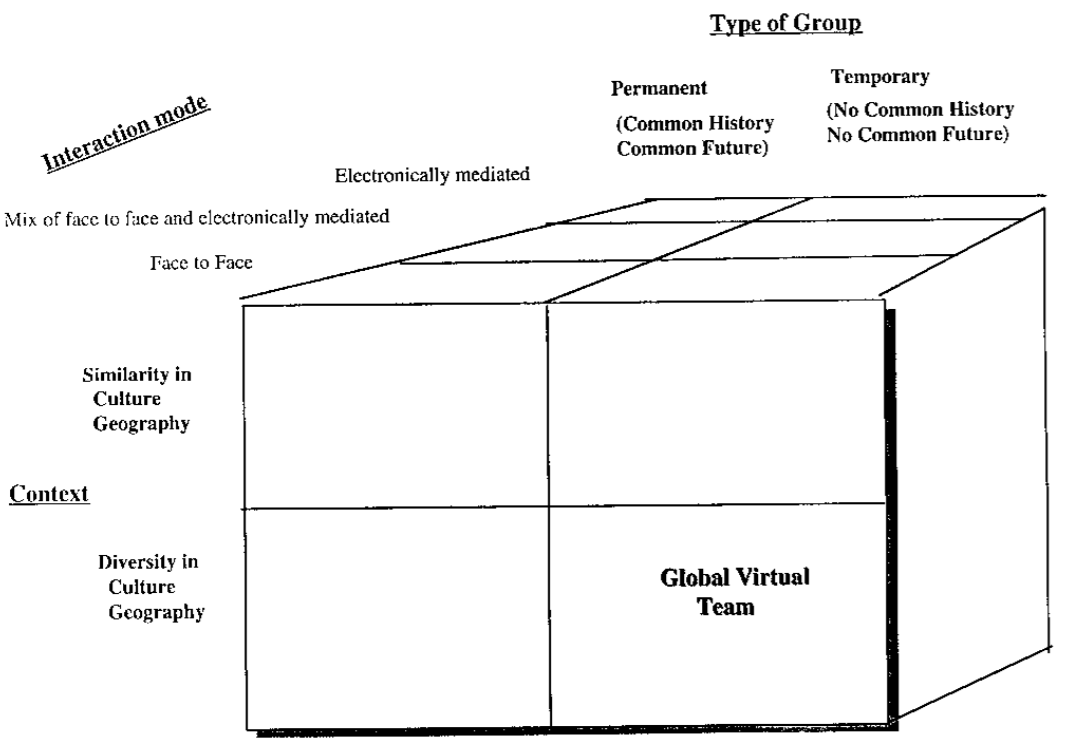
\includegraphics[width=\linewidth]{Abbildungen/GlobalVirtualTeam.PNG}	
			\caption[Virtuality of a virtual team]{Degree of virtuality that a team must reach to be considered a \textit{virtual team} \citep{jarvenpaa1999communication}.}
			\label{virtualTeamsVirtuality}
\end{figure}

Members of a \textit{virtual team} have fewer opportunities to see each other, interact or resolve conflicts, unlike traditionally formed teams. Respect and trust are the basic building blocks of a \textit{virtual team}. The effectiveness of a team is a direct consequence of this \citep[p. 378]{ren2007applying}.

\paragraph{VIRTUAL TEAMS AND TEAMEFFECTIVENESS}

Schweitzer et al. \citep{schweitzer2010conceptualizing} assumes that traditionally formed teams are more effective than \textit{virtual teams} and that \textit{team effectiveness} decreases the higher the degree of virtuality (see \textit{fig \ref{virtualTeamsVirtuality}}).
This opinion is also shared by Becker et al. According to them, the exchange of information content and the building of trust suffers due to increasing virtuality and the same effectiveness as in a face-to-face team cannot be achieved \citep{becker2002fuhrung}.

Previous studies have found positive correlations \citep{davis2000trusted}, no correlations \citep{hertel2004managing}, and negative correlations \citep{dirks1999effects} between trust and \textit{team effectiveness} in \textit{virtual teams}.

Despite the contradictory results of studies, the general opinion is that trust has a positive influence on \textit{team effectiveness} \citep{en2016trust}. 
Trust in one's team helps to block out one's own uncertainties in order to work more safely and effectively \citep{de2010does}. Furthermore, existing trust in one's team creates a greater interest in the team members, which unlocks synergy effects and enables more direct and effective interaction \citep{dirks1999effects}. 

\subsection{AVATARS AND TRUST}
George et al. \citep{george2018trusting} analyzed in their research whether more trust can be established with human-like or robotic avatars in a shared virtual environment. They found no significant difference in trustworthiness. However, a greater sense of commonality was found when interacting with a human-like avatar.

Riedl et al. \citep{riedl2014trusting} conducted a study on trust building among humans compared to avatars with human-like faces. They found that people find it easier to trust a real person than an avatar with a human-like face. According to them, trust is built between humans at the same rate as between humans and avatars.
This assumption was also confirmed by Bente et al. \citep[S. 54-59]{bente2004social}. They found that in a \textit{shared-virtual-environment} less \textit{cognitive trust} is built up towards avatars than in face-to-face, telephone and chat communications.

\section{METHODS}

A \textit{A/B testing} in combination with an inductive quantitative research design was chosen.
Group A was assigned the condition humanlike, while group B was assigned the condition non-humanlike. Participants were randomly assigned to groups and conditions. 

The analyses in this study were conducted at different levels.
Since participants work as a team and different teams have different conditions, some correlations are conducted at \textit{condition level} and some are conducted at \textit{team level}.

The \textbf{individual level} is about an individual person, while the \textbf{condition level} distinguishes between the conditions \textit{humanlike} and \textit{non-humanlike}.

The condition level can be divided into teams of 3 persons each. This division is called \textbf{TeamLevel} and it possible to make assumptions about the team. 
The \textit{Figure \ref{DifferentLevels}} shows the hierarchy of the different levels.

\begin{figure}[h]
  \centering
 		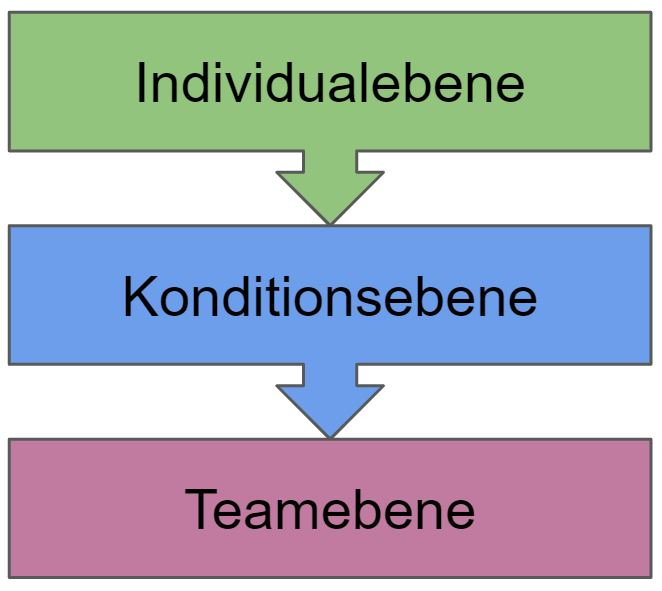
\includegraphics[width=0.5\linewidth]{Abbildungen/DifferentLevels.JPG}	
			\caption[The hierarchy levels]{The hierarchy of individual-level, condition-level and team-level.}
			\label{DifferentLevels}
\end{figure}	
	
Using a self-constructed theory-based framework (see \textit{Figure \ref{Trial Hypotheses}}), the following hypotheses were formulated :

\textbf{H1$_{1}$}: The mean values of the obtained \textit{cognitive confidence scores} differ significantly from each other between the \textit{humanlike} and \textit{non-humanlike} conditions.

\textbf{H2$_{1}$}: The higher the achieved \textit{general trust score} of a person, the higher the achieved \textit{cognitive trust score} of a person.

\textbf{H3$_{1}$}: The correlation between the \textit{cognitive trust score of teams} and the \textit{team effectiveness} with the condition \textit{humanlike} is stronger than that of teams with the condition \textit{non-humanlike}.

\textbf{H4$_{1}$}: The mean values of \textit{team effectiveness} differ significantly from each other between the \textit{humanlike} and \textit{non-humanlike} conditions.

\textbf{H5$_{1}$}: The correlation between the \textit{general trust score of a team} and the \textit{team effectiveness} with the condition \textit{humanlike} is stronger than that of teams with the condition \textit{non-humanlike}.

\begin{figure}[H]
		\begin{footnotesize}
			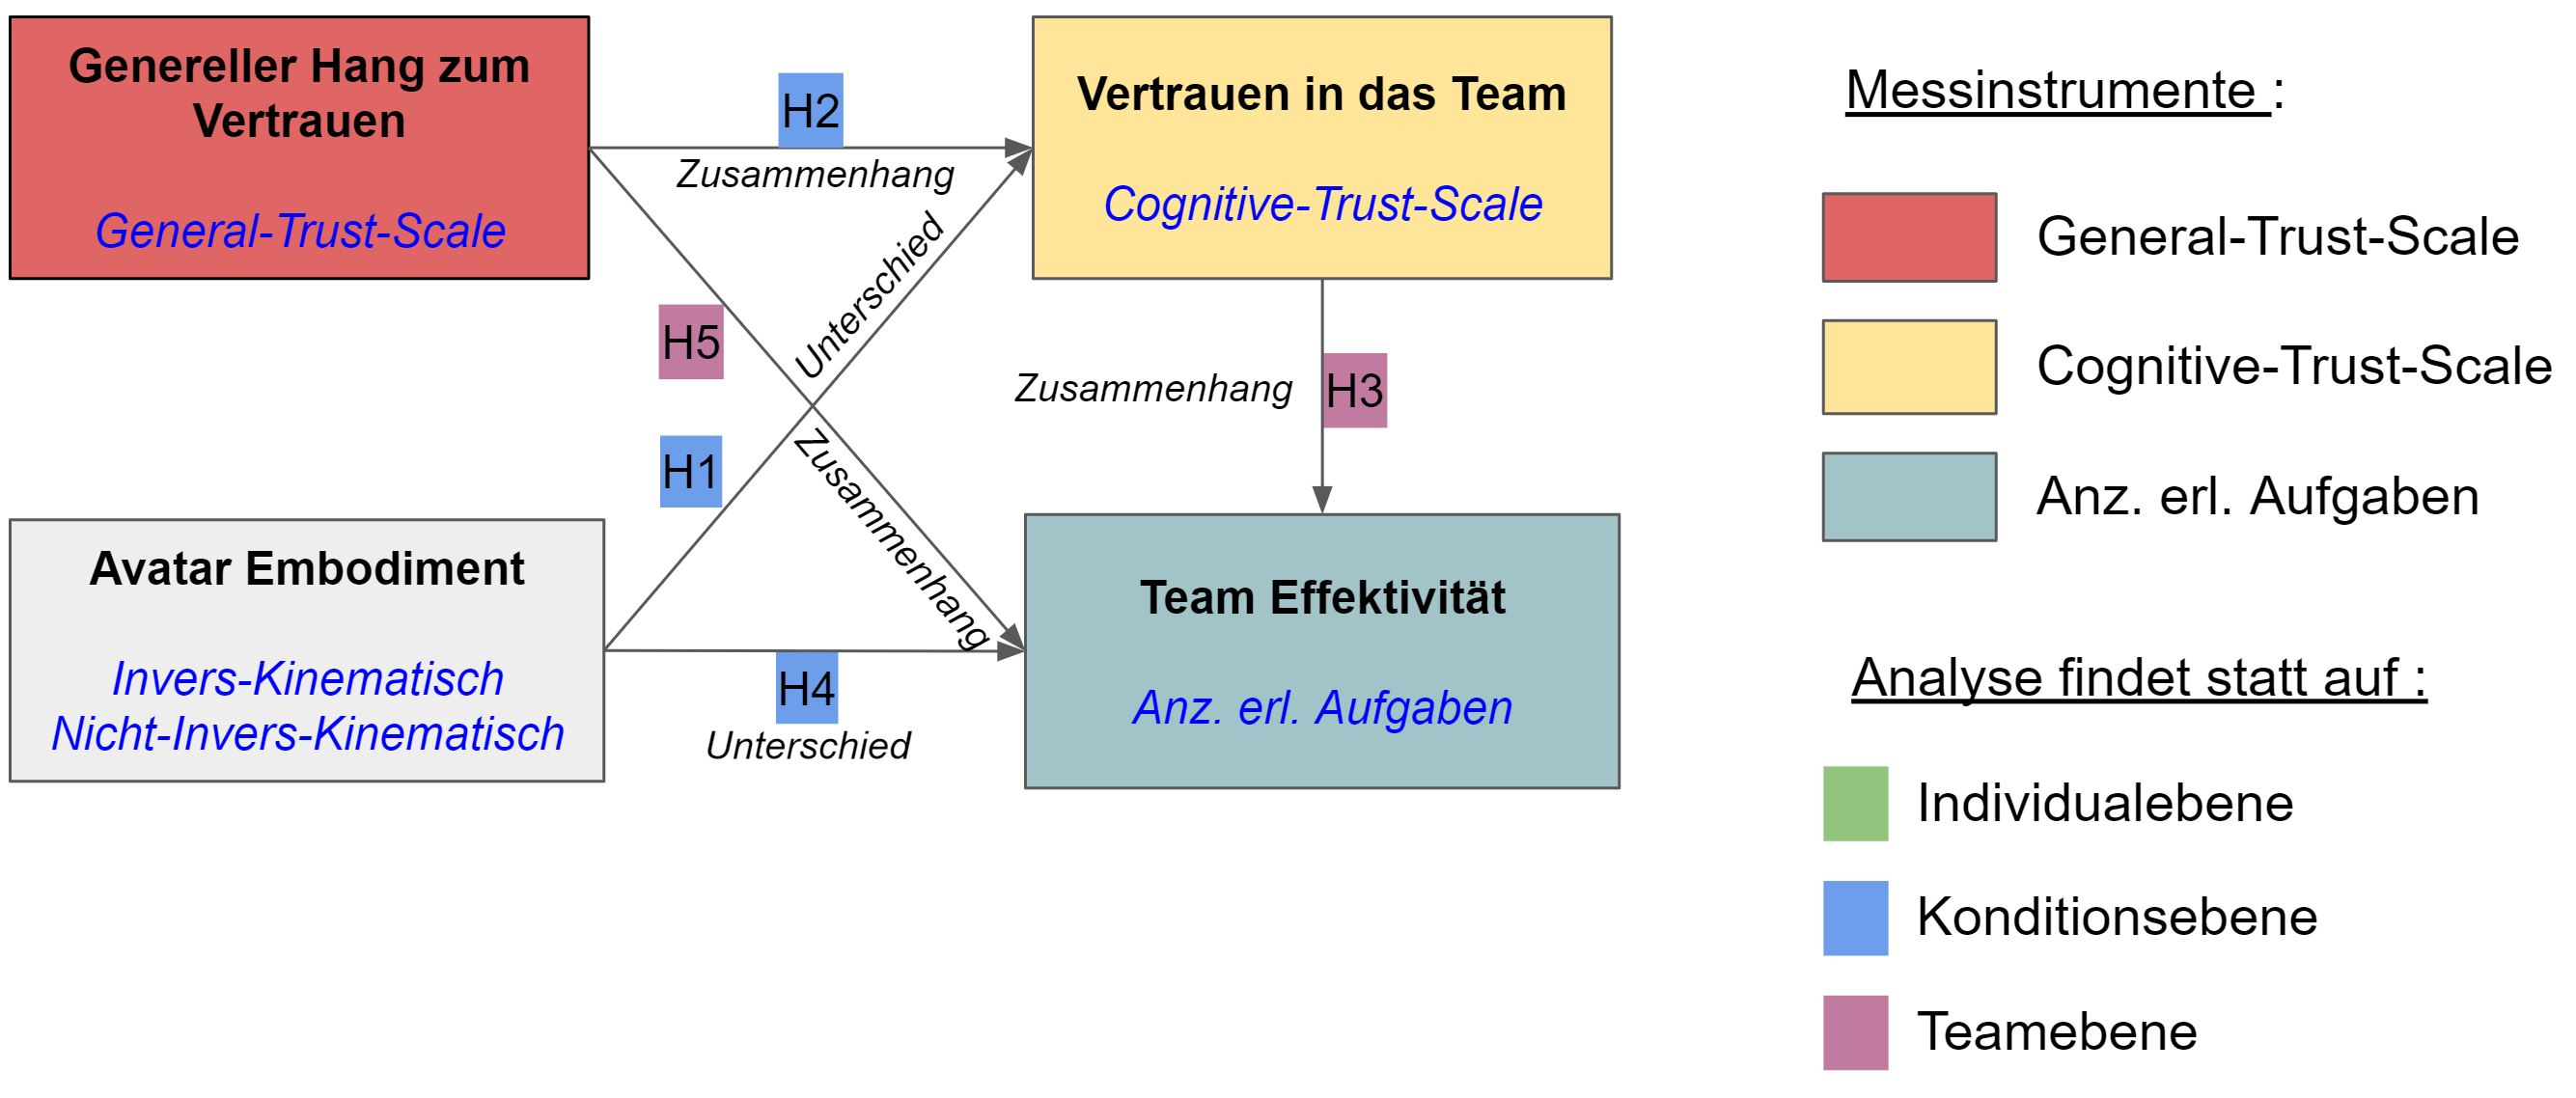
\includegraphics[width=\linewidth]{Abbildungen/Versuchshypothesen_02.JPG}		
			\caption[The self-constructed framework of experimental hypotheses]{This framework illustrates the interrelationships of the posed hypotheses.}
			\label{Versuchshypothesen}
		\end{footnotesize}
	\end{figure}	

General trust in this study refers to the extent to which participants tend to give others the benefit of the doubt. \citep[S. 30]{mcallister1995affect}.
\textit{Cognitive trust} refers to \textit{conviction} in the abilities or in the reliability of another \citep[S. 30]{mcallister1995affect}.
The \textit{team effectiveness} is measured by the number of rounds completed by the team during the experiment.

%\subsection{MEASURING METHODS}
\begin{table*}
  \caption{MEASURING METHODS}
  \label{tab:commands}
  \begin{tabular}{llcr}
    \toprule
    Scale & What was measured? & $\alpha$ & Likert-Points \\
    \midrule
    \texttt{General-Trust-Scale \citep{couch1996assessment}} & General trust value of the individual participants & ,91 & 1-7 \\
    
    \texttt{Cognitive-Trust-Scale  \citep[S. 37]{mcallister1995affect}} &Built up \textit{cognitive trust} during the experiment & ,91 & 1-5\\
    
     \texttt{\textit{Quality of team communication} \citep[S. 1049]{gonzalez2014climate}} & Perceived quality of team communication & ,76 & 1-5 \\
     
      \texttt{\textit{Perceived team effectiveness}\citep[S. 469]{gibson2003team}} & Extent of perceived team effectiveness & ,62-,88 & 1-7\\
          
       \texttt{NASA-TLX\citep{NASATLX}} & Task load during the experiment & ,84 &1-21  \\
       
       \texttt{IPQ \citep{IPQ}} & The sense of presence & ,85 & 1-7 \\
       
        \texttt{\textit{Co-Präsenz} \citep[S. 487]{nowak2003effect}} &  Co-, Social-, Telepresence & ,78-,90 & 1-7; 1-10 \\
    \bottomrule
  \end{tabular}
\end{table*}

\subsection{PARTICIPANTS}

The participants were acquired in two ways. On the one hand, people in the circle of acquaintances were approached, who would be provided with the necessary hardware. Secondly, participants were sought in various forums (e.g. VRForum.de, Computerbase.de, Hardwareluxx.de, etc.). Furthermore, participants were acquired with the help of various social networks related to VR as well as random WhatsApp chat groups with 50 or more members.

To participate in the experiment, participants needed a fully functioning SteamVR, Windows Mixed Reality, or Oculus Rift/Rift-S head-mounted display with compatible controllers, as well as a powerful VR-enabled PC. The experimenter used a PC without a head-mounted display to control and manage the experiment from outside.

\subsection{PROCEDURE AND IMPLEMENTATION}
To conduct the experiment, a shared virtual environment was developed in which three team members could see each other as avatars and interact with each other. The shared virtual environment has been developed with Unity 2019.4.3f1 and the HD render pipeline. To ensure real-time communication between clients, the multiplayer framework \textit{Normcore v2.0}\footnote{www.Normcore.io} was used.

Three people were placed in each time slot to form a team. The participants were \textit{not} introduced face-to-face and saw themselves only as a representation of an avatar.
The test lasted 35 minutes and was divided into
		\begin{itemize}
			\item 5 minutes pre-questionnaire,
			\item 5 minutes video explanation,
			\item 10 minutes experiment,
			\item 15 minutes post-questionnaire.
		\end{itemize}
The pre-questionnaire was used to collect general demographic data from the participants. The explanatory video showed all the relevant mechanics of the experiment. Furthermore, the video explanation ensured that all participating individuals had the same level of information about how the experiment was conducted. During the experimental session, participants had 10 minutes to complete as many rounds as possible as a team. Over the subsequent post-questionnaire, all relevant questionnaires were processed for statistical analysis of the experimental hypothesis. The maximum test duration after starting the experiment was 600 seconds and a maximum of 15 rounds could be completed. The rounds became incrementally more difficult every third round as one symbol was added to the pool of symbols to be guessed.
\textit{Figure \ref{RoundDifficulty}} shows the increasing round difficulty used to measure \textit{team effectiveness} in this experiment.

\begin{figure}[H]
		\begin{footnotesize}
		\centering
			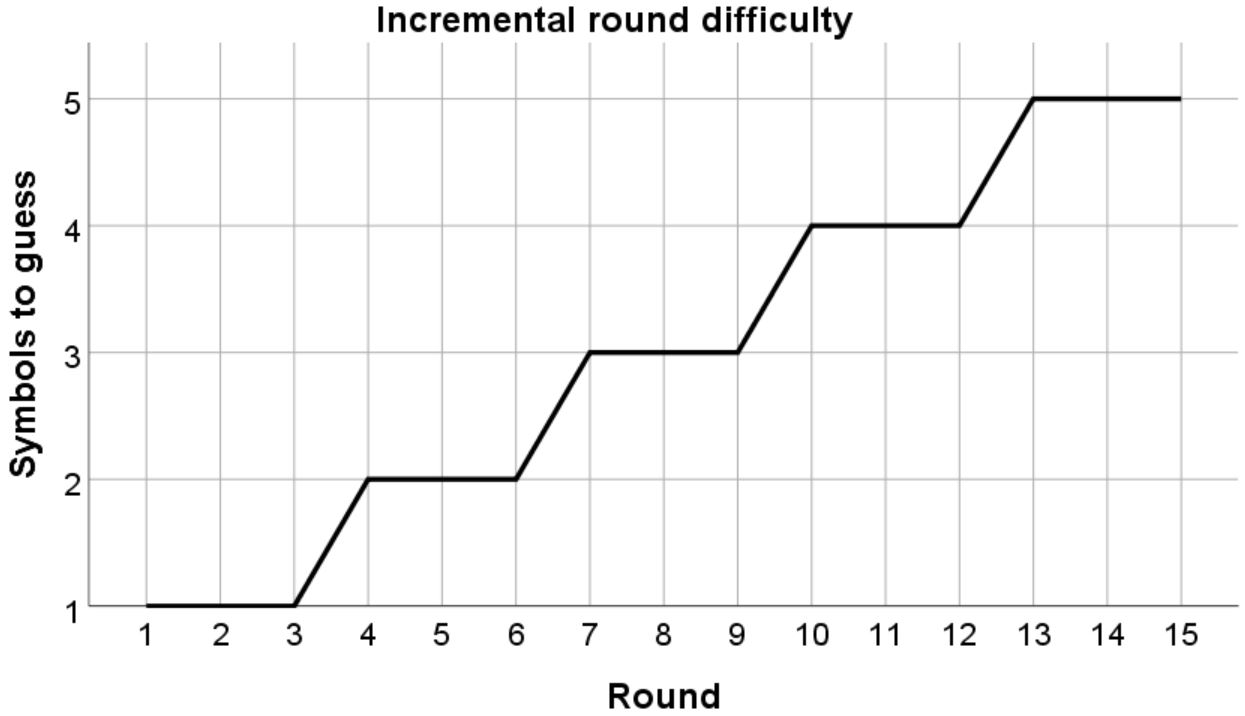
\includegraphics[width=0.7\linewidth]{Abbildungen/RoundDifficulty.JPG}	
			\caption[The difficulty of the rounds]{The increasing difficulty of the symbols to be guessed in the rounds. In rounds 1-3 one symbol had to be guessed, in rounds 3-6 two symbols and so on.}
			\label{RoundDifficulty}
		\end{footnotesize}
	\end{figure}

\subsection{Detailed test execution}
At the beginning of each new round, players were assigned the color black, green or red.
The player marked black has the task of explaining to his teammates the symbols that are color-coded for him. The other team members had the task to identify the symbols shown by the black player by gesticulation and to log them on their podium. The goal was to correctly identify as many symbols as possible, thereby advancing to higher rounds together.

The symbols on the podium of the player marked in black were color-coded either green, red or green-red. The podiums of the other players also had symbols on them, but these were arranged randomly and had no color markings. The player marked in black now tried to explain the symbols marked in the respective player color in front of him to the other players marked with red and green. If the player just addressed by the black player believed to have recognized a symbol, he logged the symbol by pressing down the matching button on his podium. 

If all the marked symbols were successfully identified and logged in, a bright green ball appeared, indicating the end of a round.
In the next round, another player was clearly marked with black, red or green.
\textit{Figure \ref{AvatareImEinsatz}} shows both avatar conditions \textit{humanlike} (a) and \textit{non-humanlike} (b) during the experimental procedure.
	
\begin{figure}[h]
  \centering
  \subfloat[][]{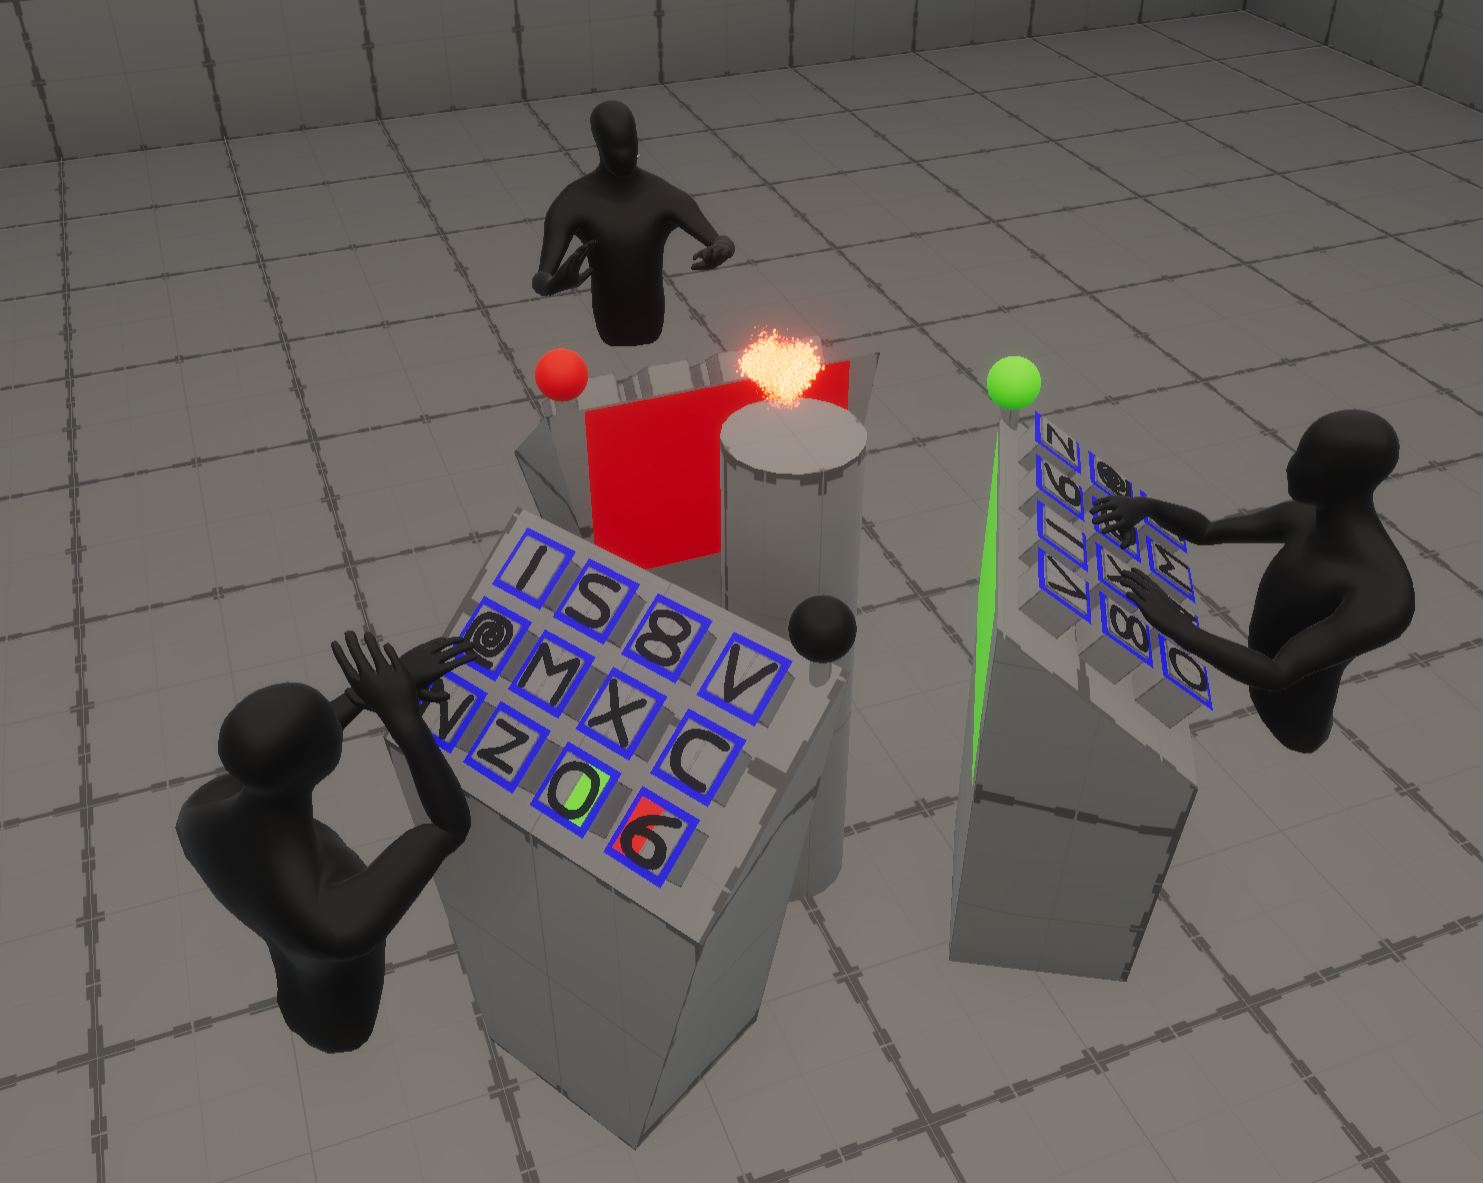
\includegraphics[width=0.45\linewidth]{Abbildungen/Podeste_IK_Avatars.jpg}}
  \qquad
  \subfloat[][]{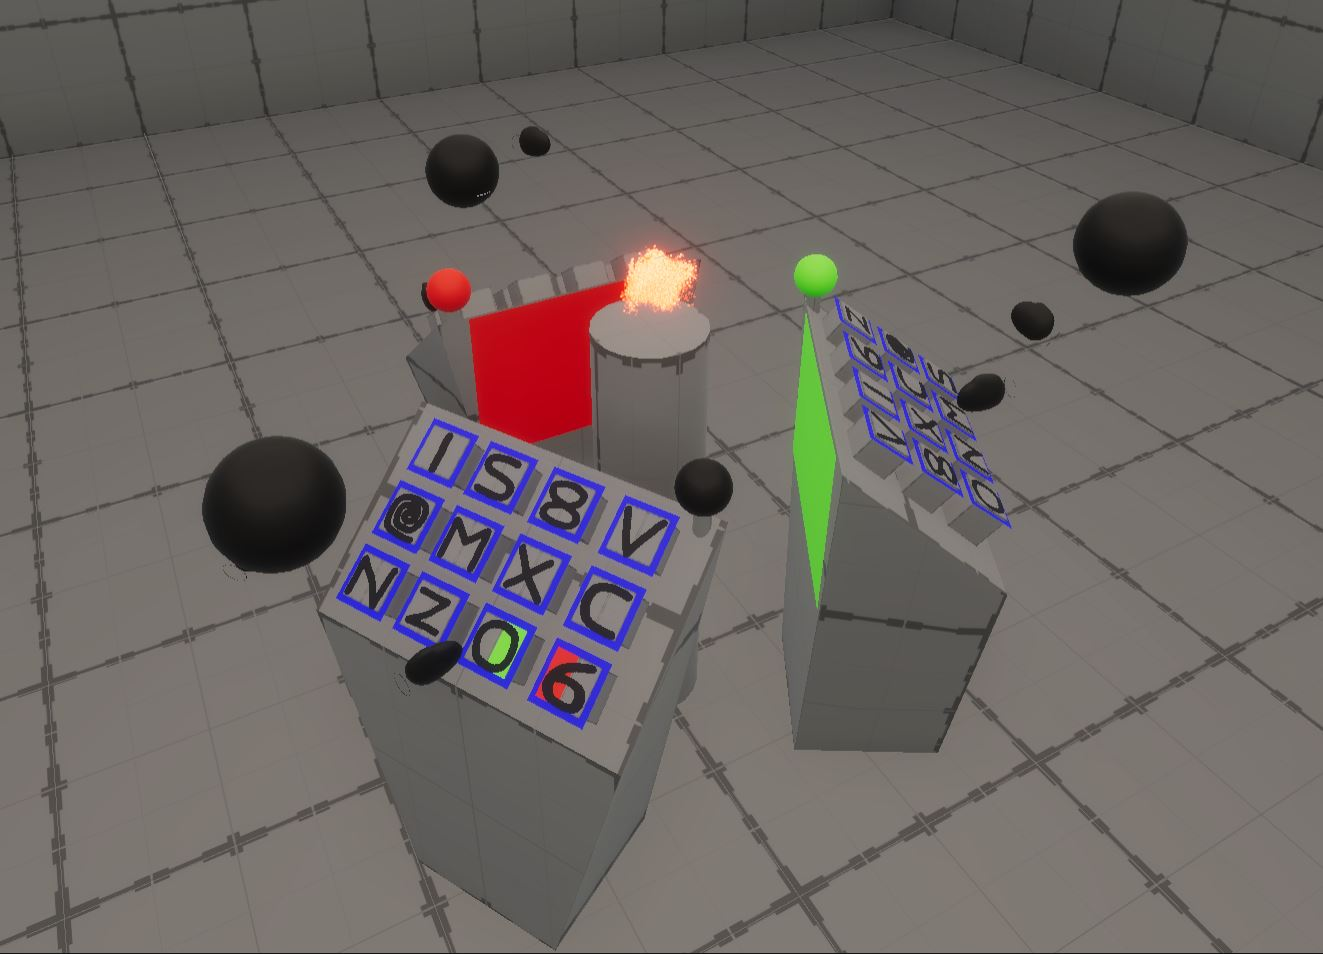
\includegraphics[width=0.45\linewidth]{Abbildungen/Podeste_Non_IK_Avatars.jpg}}
  \qquad
  \subfloat[][]{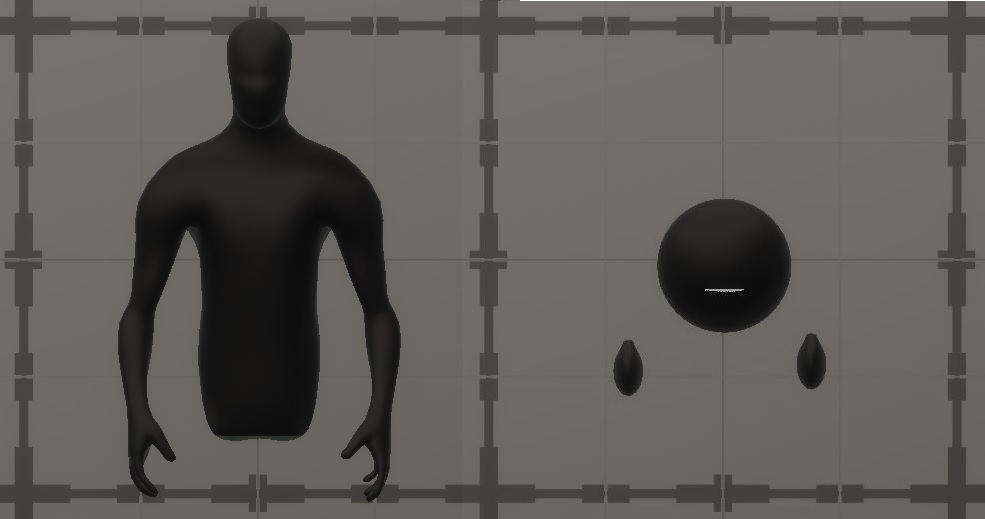
\includegraphics[width=0.45\linewidth]{Abbildungen/Avatars.JPG}}
  \caption[The avatars in the experimental environment]{Avatar conditions \textit{humanlike} (a) and \textit{non-humanlike} (b) during the execution of the experiment. (c) shows the avatars used side by side. Left: \textit{humanlike} avatar and right: \textit{non-humanlike} avatar.}
  \label{AvatareImEinsatz}
\end{figure}

\section{RESULTS}
\subsection{HYPOTHESIS}
%H1
Based on the statistical analysis of Hypothesis 1, it can be concluded that different avatar conditions have a \textit{significant} influence on the formed \textit{cognitive trust} (Mann-Whitney-U $U = 64.000; Z = -2.029; p =.042 < \alpha =.05; r =-.370$). Thereby, participants with the condition \textit{non-humanlike} $(\bar{x} = 4.622)$ formed more \textit{cognitive trust} than participants with the condition \textit{humanlike} $(\bar{x} = 4.188)$. 

%H2
Through the analysis of Hypothesis 2, \textit{no evidence} could be found that there is a \textit{significant} correlation between \textit{general trust} and \textit{cognitive trust}. 

%H3
Contrary to the assumption of Hypothesis 3, a \textit{significant} relationship was found between the formed \textit{cognitive trust in the team} and the \textit{team effectiveness} with the condition \textit{non-humanlike} (Spearman-Rho $r =.975$; $p =.005 < \alpha = .05$). This correlation differs according to Fisher Z-score for independent samples ($Z=-1.977$), \textit{significant} ($p =.024 < \alpha = .05$) from that of the condition \textit{humanlike}.
 
%H4
During the analysis of Hypothesis 4, it was found that \textit{team effectiveness} \textit{not significant} differs from each other due to different avatar conditions (Mann-Whitney U $U = 103.500; Z = -.377; p =.706 > \alpha = .05; r = -.060$). An average team effectiveness of $\bar(x) = 9$ was found for both avatar conditions.

%H5
Furthermore, based on the analysis of Hypothesis 5, there is \textit{no evidence} that there is a \textit{significant} correlation between a person's \textit{propensity to trust} and \textit{team effectiveness} in a \textit{virtual team}.

Während der Analyse der subjektiven Daten wurde ein \textit{signifikanter} Unterschied der Mittelwerte der Teamkommunikation (Mann-Whitney-U : $U = 63,500; Z = -2,062; p =,039 < \alpha = ,05$)  auf Konditionsebene festgestellt. Der Mittelwert der \textit{Teamkommunikation} der Kondition \textit{humanlike} beträgt $\bar{x} = 4.013$, während der Mittelwert der Teamkommunikation der Kondition \textit{non-humanlike} $\bar{x} = 4,48$ beträgt. Bei beiden Konditionen ist die Tendenz einer hohen Teamkommunikation ersichtlich ($\bar{x} = 4,013$; $\bar{x} = 4,48$ $ > \bar{x}  = 3$).
 
Zudem kann festgehalten werden, dass sich ein erhöhtes Präsenz-Gefühl (Präsenz, Telepräsenz, selbst wahrgenommene Co-Präsenz, wahrgenommene Co-Präsenz des anderen und Soziale-Präsenz) auf Konditionsebene während der Versuchsdurchführung gebildet hat. Die allgemeine Belastung lag unter dem Durchschnitt der möglichen anzugebenden Werte und die wahrgenommene Teameffektivität war überdurchschnittlich hoch.
Weiterhin gibt es einen \textit{signifikant} positiven Zusammenhang zwischen dem \textit{kognitiven Vertrauen} und der \textit{wahrgenommenen Teameffektivität}  (Spearman-Rho : ($r =,869; p =,000 < \alpha = ,05$) und der \textit{Teamkommunikation} ($r =,676; p =,006 < \alpha = ,05$) auf Konditionsebene bei der Kondition \textit{non-humanlike}.

\subsection{SUBJECTIVE DATA}


Das von allen Teilnehmern durchschnittlich angegebene \textit{Gefühl der Präsenz} kann mit dem Wert $\bar{x} = 4,446$ als stark interpretiert werden ($\bar{x} > 3,5$). Die \textit{Telepräsenz} ($\bar{x} = 5,286$) sowie die \textit{soziale Präsenz} ($\bar{x} > 6,409$) werden etwas stärker als durchschnittlich empfunden und deuten dadurch auf ein höheres Gefühl der Anwesenheit sowie auf ein stärkeres Gefühl der Nähe zwischen den Teilnehmern hin. Auch die \textit{selbst wahrgenommene Co-Präsenz} sowie die \textit{wahrgenommene Co-Präsenz des anderen} liegen mit den Werten $\bar{x} = 3,827$ und $\bar{x} = 3,877$ über dem Mittelwert der Antwortmöglichkeiten ($\bar{x} > 2,5$) und weisen somit eine Tendenz zur starken \textit{Co-Präsenz} auf.

Daneben liegt die durchschnittlich \textit{wahrgenommene Teameffektivität} mit dem Wert $\bar{x} > 4,886$ über dem Wert 3,5 und lässt sich somit im Bereich der als eher stark empfundenen Teameffektivität ($3,5 - 7$) verorten.
Die Werte des NASA-TLX (Allg. Anstrengung) ($\bar{x} < 7$) zeigen, dass das VR Experiment als mittelmäßig bis wenig anstrengend wahrgenommen wurde ($\bar{x} < 11$ ).

Auf Konditionsebene ist eine signifikante ($r =,869; p =,000 < \alpha = ,05$) starke positive Korrelation (vgl. \citep{cohen2013statistical}) mit dem Spearman- Korrelationskoeffizient  zwischen den \textit{kognitiven Vertrauenswerten} und \textit{der wahrgenommenen Teameffektivität} der Kondition \textit{non-humanlike} zu erkennen.

Weiterhin ist eine signifikante ($r =,676; p =,006 < \alpha = ,05$) positive Korrelation starken Effektes (vgl. \citep{cohen2013statistical}) zwischen den \textit{kognitiven Vertrauenswerten} und der \textit{Team-Kommunikation} der Kondition \textit{non-humanlike} auf Konditionsebene zu erkennen.

\section{DISCUSSION}
\subsection{Building trust through the avatar conditions}
Die Ergebnisse des Experiments widersprechen der Untersuchung von Bente et al. (vgl. Kapitel \ref{AvatarTrust}), die vermuten ließ, dass bei der Kondition \textit{humanlike} ein größerer \textit{kognitiver Vertrauensaufbau} stattfindet als bei der Kondition \textit{non-humanlike} (Hypothese 1). Es ist laut der statistischen Auswertung genau das Gegenteil der Fall, denn die Teilnehmer mit der Kondition \textit{non-humanlike} erzielen im Durchschnitt einen signifikant höheren kognitiven Vertrauenswert.
Ein Grund für dieses Ergebnis könnte sein, dass der verwendete \textit{humanlike}-Avatar vom \textit{Uncanny Valley Effekt} \footnote{Der Uncanny-Valley Effekt beschreibt das Gefühl des Unbehagens ab einem gewissen Realitätsgrad  \citep[S. 352-353]{gast2011unheimliche}.} betroffen ist.
Weiterhin könnte die in diesem Experiment verwendete Inverse-Kinematik, als fremdartig empfunden worden sein. Auch dadurch falsch interpretierte Gestikulation kann zu einem geringeren Vertrauensaufbau in das jeweilige Gegenüber geführt haben.

\subsection{Building trust through the general trust}
Dass kein signifikanter Zusammenhang zwischen dem \textit{kognitiven Vertrauen} und dem \textit{generellen Vertrauen} bei unterschiedlichen Avatar- Konditionen besteht (Hypothese 2), kann auch als Vorteil gesehen werden.
So lässt sich vermuten, dass es während einer kurzfristigen Zusammenarbeit in einem Shared-Virtual-Environment nicht von Relevanz ist, wie hoch oder niedrig das \textit{generelle Vertrauen} einer Person ist. 
Da nur die unterschiedlichen Avatar-Konditionen einen signifikanten Einfluss auf die Bildung des kognitiven Vertrauens besitzen, kann davon ausgegangen werden, dass das \textit{generelle Vertrauen} während einer Kennenlernphase eines virtuellen Teams keine größere Rolle spielt und isoliert betrachtet werden kann.

\subsection{Trust in the team and team effectiveness}
Die Hypothese 3, in der vermutet wurde, dass der Avatar mit der Kondition \textit{humanlike} mehr \textit{kognitives Vertrauen} aufbaut, muss ebenfalls abgelehnt werden. Jedoch wurde während der Analyse dieser Hypothese festgestellt, dass es einen \textit{signifikanten Zusammenhang} zwischen dem gebildeten \textit{kognitiven Vertrauen} und der \textit{Teameffektivität} der Kondition \textit{non-humanlike} gibt. Da die Hypothese 4 nicht angenommen werden kann, jedoch ein signifikanter Zusammenhang mit der Kondition \textit{non-humanlike} bei der Analyse der Hypothese 3 festgestellt wurde, muss vermutet werden, dass die Ergebnisse der Hypothese 3 und Hypothese 4 entweder zufälliger Natur sind oder die Messung der Teameffektivität verbessert werden muss.
Die kleine Stichprobengröße der Studie könnte zudem eine Ursache dafür sein, dass die Ergebnisse von Hypothese 3 und Hypothese 4 keine eindeutigen Ergebnisse liefern. Bei einer deutlich größeren Stichprobengröße könnte bei einer größeren Varianz der \textit{Teameffektivitätswerte} gegebenenfalls ein signifikanter Unterschied oder ein eindeutiger signifikanter Zusammenhang mit dem \textit{kognitiven Vertrauen} und der \textit{Teameffektivitätswerte}, festgestellt werden.

\subsection{LIMITATIONS}
Als technische Limitation dieser Arbeit kann die eingesetzte Technik der Gestikulation aufgeführt werden. Die unterstützten Head-Mounted-Displays boten keine Möglichkeit, die Finger oder die gesamten Hände in der Virtual-Reality abzubilden. Die Verständigung innerhalb des Shared-Virtual-Environment kann durch den Einsatz von Finger- und Handtracking intensiviert werden, da verschiedene Gesten genauer wiedergegeben werden können. Das Finger- und Handtracking ist beispielsweise durch eine Oculus Quest oder Oculus Quest 2 möglich. Ein weiterer Aspekt, um die Menschenähnlichkeit und den Realismus bei der Avatar-Kondition \textit{humanlike} zu erhöhen, wäre der Einsatz von Mimik.
Eine weitere Limitierung dieser Untersuchung war, dass die Teilnehmer bevor das Experiment startete wussten, dass diese in einem Shared-Virtual-Environment mit realen Personen agieren würden. 
Darüber hinaus ist der Avatar mit der Kondition \textit{humanlike} in dieser Studie nicht auf Menschenähnlichkeit, Realismus oder Ähnliches überprüft worden. 
\section{CONCLUSION AND FUTURE WORK}
Shared-Virtual-Environments entwickeln sich aktuell sehr rasant. Die Coronapandemie hat gezeigt, dass virtuelle Kollaborationsmaßnahmen einen großen Einfluss auf Unternehmen weltweit haben. Es ist mehr Forschung darüber nötig, wie Teams effektiv in einem Shared-Virtual-Environment zusammenarbeiten können.

Es könnte nicht nur untersucht werden, welche Art eines Avatars in einem Shared-Virtual-Environment mehr Vertrauen schafft oder mehr \textit{Teameffektivität} erzeugt, sondern auch, wie die eingesetzte Sprache, die Mimik, die Gestik, die Größe, das Geschlecht oder der vorherige Bekanntheitsgrad der Personen sich auf das Vertrauen und die \textit{Teameffektivität} auswirkt.
Weiterhin könnte untersucht werden, wie die Art und Dauer der Nutzung des Head-Mounted-Displays, während ein Team zusammenarbeitet, sich auf das Vertrauen ins Team und die Teameffektivität auswirkt.

Eine Weiterführung dieser Studie könnte untersuchen, in welchem Maß sich der \textit{kognitive Vertrauensaufbau im Team} ändert, je nachdem, ob die Teilnehmer wissen, dass sie mit Menschen zusammenarbeiten oder nicht. Darüber hinaus wäre es interessant zu untersuchen, wie sehr sich der Unterschied zwischen einer verbalen und einer nonverbalen Kommunikation auf das gebildete Vertrauen im Team in einem Shared-Virtual-Environment auswirkt.  
Weiterhin könnten ähnliche Studien durchgeführt werden, bei denen die einzelnen Runden der Kollaborationsaufgabe schneller hintereinander ausgeführt werden oder die Avatare ein anderes Aussehen besitzen.

Es konnte ein signifikanter Unterschied beim gebildeten \textit{kognitiven Vertrauen} zwischen den Avatar-Konditionen festgestellt werden, wobei sich mehr \textit{kognitives Vertrauen} bei den nicht- menschenähnlichen Avataren bildete. Es konnte jedoch kein statistisch signifikanter Unterschied zwischen den Avatar-Konditionen und der \textit{Teameffektivität} festgestellt werden. Weiterhin zeigen die Ergebnisse keinen signifikanten Zusammenhang zwischen dem \textit{generellen Vertrauen} und dem gebildeten \textit{kognitiven Vertrauen} einer Person. Zwischen dem \textit{kognitiven Vertrauen} und der \textit{Effektivität eines Teams} konnte ein signifikanter Zusammenhang bei der Kondition \textit{humanlike} festgestellt werden.

In einem virtuellen Team besitzt die Avatar-Kondition laut dieser Studie somit keinen eindeutigen Einfluss auf die \textit{Teameffektivität}. Es kann jedoch sinnvoll sein, den Avatar nicht zu menschenähnlich zu gestalten, um mehr \textit{kognitives Vertrauen} zu bilden.
%Es empfiehlt sich, diese Studie mit einer großen Stichprobe zu replizieren und die Einflüsse anders gestalteter Avatare zu untersuchen. 
Die Arbeit in einem virtuellen Team muss folglich nicht mit aufwendig gestalteten Avataren unterstützt werden. So können beispielsweise Unternehmen, die mit virtuellen Teams in einem Shared-Virtual-Environment arbeiten wollen, auf simple Avatar-Modelle zurückgreifen, um den Vertrauensaufbau im Team zu unterstützen.

%%
%% The next two lines define the bibliography style to be used, and
%% the bibliography file.
%\citestyle{acmauthoryear}
\bibliographystyle{ACM-Reference-Format}

\bibliography{sample-base}

%%
%% If your work has an appendix, this is the place to put it.
\appendix


\end{document}
\endinput
%%
%% End of file `sample-sigconf.tex'.
